\chapter{Sharing Data Continuum} % Main chapter title
\label{ch:data} % Change X to a consecutive number; for referencing this chapter elsewhere, use \ref{ChapterX}

This chapter address the surrounding environment around the user in terms of the Social AR Continuum. The surrounding environment level-of-details can determined based the relationship between the user and the social contact that we're sharing the environment with. 
The aim of this chapter is to answer the research question \textit{RQ3: "How to share virtual objects/data with our social network through wearable AR"}
In this chapter we study different ways for sharing the surround environment (360 Panoramas \ref{sec:surrounding:360}, 3D scanned surroundings \ref{sec:surrounding:environment}). We also look into partially sharing/hiding \ref{sec:surrounding:hiding} part of the room with social contacts. For each way of sharing, we discuss levels of details that can be shared based on user relationships. 

\section{Filtering Shared Social Data}
\label{sec:surrounding:360}

The social data describing the surrounding scene can described in different levels of detail. A different ways of describing a surrounding scene include: a 2D image, a panoramic image, a video, a 360-degrees video, a 3D depth image, or a VR 3D model. These different ways of describing the same scene represent the levels of details that can be varied based on the Social AR Continuum and the social proximity between the social contacts. 

This section describes a method and a prototype implementation for filtering shared social data (e.g., 360-degree videos) using wearable AR devices (e.g., HoloLens) \cite{Nassani2018a}. The data filtering is based on the sharer-viewer relationships in order to preserve privacy. For example, when sharing a 360-degrees video, if the user has an intimate relationship with the viewer, then the full fidelity (i.e., the whole 360-degree video) of the user's environment is visible. However, if the two are strangers, then only a snapshot image is shared, and the user cannot get more information about the sharer's environment. By varying the fidelity of the shared content, the viewer can focus more on the data shared by their close relations and differentiate this from other content. Also, the approach enables the sharing-user to have more control over the fidelity of the content shared with their contacts for privacy.

% In this work, we are trying to answer the question, what would be the best way to share rich data (such as 360 videos) within a large social network? The hypothesis is that filtering data based on the user-viewer relationship or proximity will increase the feeling of being together or inter-connectedness. 


% =============================================================================
\subsection{Sharing Social Data}
% =============================================================================

From the perspective of the person who is sharing the data (the sharer) with their social contacts (Figure \ref{fig:data:sharer}), the data is collected in its highest fidelity (e.g., a fully spherical 360-degree view) which will be shared with those viewers with the closest (most intimate) social relationships. For less-intimate friends, a 2D video, extracted from the 360 videos based on the sharer's view direction over time, will be shared. For Strangers, the sharer can select which snapshot image from the 2D video sequence to display. The central metaphor is that the closer the relationship that the user has to the viewer, the richer data that they can share from their point of view (360-degree videos, 2D videos, still images).

\begin{figure}[ht]
    \centering
    \includegraphics[width=1.5in]{images/chi/images-04.eps}
    \caption{Sharing point of view with different fidelity of representation.}
    \label{fig:data:sharer}
\end{figure}

An example use-case scenario for filtering by sharer is where the sharer is going on a hike and wanting to share the experience of being in an interesting place such as near a river. The sharer takes a live 360-degree video of the surrounding environment and shares it with her followers. The sharer then gets to see how the followers are able to see the shared data based on their social relationship to her. The sharer's intimate friends and family will see the live 360-degree video, other friends the 2D video, and strangers still images of the scene, all automatically created from the 360-degree video recording.

% =============================================================================
\subsection{Viewing Shared Social Data}
% =============================================================================

The user viewing the shared data (the viewer) uses a wearable AR interface to see content from their social network superimposed over the real world, based on proxemics. For example, the viewer may be interested in seeing what their social contacts (followers) are up to and the places they have been. In this scenario the viewer can look around through the AR display to see their social contacts placed around them in three circles ordered by relationship. On top of each social contact, the viewer can see the content they are sharing, filtered based on the social relationship between the social contact and the viewer.

Based on our earlier work \cite{Nassani2017a}, the people who are socially closer will appear in the AR view visually closer and have a more realistic representation. The content shared by each social contact will appear above their avatar (see Figure \ref{fig:data:viewer}), and to view the content more clearly, the user can select it (e.g., using the HoloLens air-tap gesture) to bring the content closer or walk to move inside the 360-degree video sphere. The user can then tap again to bring back the content to its original place to see other social contacts. 

\begin{figure}[ht]
    \centering
    \includegraphics[width=3in]{images/chi/3_levels_of_data.png}
    \caption{Social contact sharing in different relationships with the viewer (Left to right: Intimate, Friend, Stranger). The shared data content (above the avatar) is filtered (360-degree video, 2D video, 2D image) based on social relationship.}
      \label{fig:data:viewer}
\end{figure}

In addition to this operation, this section proposes that the viewers can also see the shared content in different fidelity (360-degree videos, 2D videos or images) based on the social relationship with the sharer (Intimate, Friend or Stranger). While the sharer could restrict the fidelity of the shared content based on the social relationship as mentioned earlier, the viewer could also filter the content based on their preference. In order to avoid getting mentally overloaded by seeing too much content in high fidelity, the viewer should be able to choose the preferred fidelity for the shared content from each social contact. This could be achieved either explicitly by choosing a fidelity for each social contact, or implicitly by moving closer to or further from the avatar representing the contact.      

% =============================================================================
\subsection{Prototype}
% =============================================================================

To explore using the Social AR Continuum metaphor for sharing data between social contacts, a prototype was built using the Microsoft HoloLens. The prototype software was built using Unity 3D game engine, and it allows users to view their social contacts on a wearable AR interface. Figure \ref{fig:data:system} shows the structure of the prototype system. 

\begin{figure}[ht]
    \centering
    \includegraphics[width=3in]{images/chi/images-03.eps}
    \caption{System components.}
    \label{fig:data:system}
\end{figure}

The prototype places social contacts around the user (viewer) in three concentric circles which are controlled by the \textit{Circles Manager}. The social contacts have different visual fidelity and proximity based on their initial relationship to the viewer, and are rendered using the \textit{Avatar Controller}. The avatars were randomly pre-generated without any resemblance to actual contacts. MakeHuman\footnote{http://www.makehuman.org/} was used to generate the 3D avatars. The viewer (HoloLens user) can turn their head to face different social contacts and then use gestures (air taps) to interact with the contact (view their data or change their position which represents the social relationship). The interactions with HoloLens are enabled using the open-source library \textit{HoloToolkit}\footnote{https://github.com/Microsoft/MixedRealityToolkit-Unity}. The data content shared by the social contacts are controlled by the \textit{Data Controller} which determines which fidelity needs to be displayed based on the social relationship between the avatar and the viewer. The top-level \textit{Scenario Manager} defines the implementation needed for different conditions in the user study, including interaction with avatars, shared data and the concentric circles. 

% =============================================================================
\subsection{User Study}
% =============================================================================

A user study was conducted to test the system usability and effects on social presence, comparing the following conditions: 

\begin{itemize}
    \item C1) Baseline: Shows the shared 360-degree videos from all social contacts.
    \item C2) Tap-to-change: Filters the fidelity of the shared 360-degree videos based on the relationship between the viewer and the social contact. The user can tap on any social contact to cycle through different relationships.
    \item C3) Walk-to-change: Filter the fidelity of the shared 360-degree videos based on the physical distance between the viewer and the social contact.
\end{itemize}

The task was for participants to wear the headset and observe 12 social contacts (mocked up, not reflecting the participant's real social contacts) placed around the user at equal angles from each other to complete a circle (360 degrees) around the viewer, and at different distances to the viewer (centre) based on the social relationship. Each social contact had shared content floating above their head, filtered depending on the type of social relationship that the social contact had with the viewer. 

The participant could view the data content by performing the air-tap gesture on it. Once tapped, the content moved closer to the viewer. For instance, if the viewer tapped on the sphere of a 360-degree video, then the sphere immersed the participant to experience it, while for a 2D video, it was moved closer to the user so they could see it at full-screen resolution.

Participants were asked to answer the 5-point Likert-scale questions shown in Table \ref{tbl:questions} which are based on prior work \cite{Biocca2003}. Participants were asked to rate their experience on the Subjective Mental Effort Questionnaire (SMEQ) \cite{Sauro2009}. 

\begin{figure}[ht]
    \centering
    \includegraphics[width=1.5in]{images/chi/images-02.eps}
    \caption{Questionnaires for Social Presence including the following dimensions: CoPresence (CoP), Attentional Allocation (Atn), Perceived Message Understanding (MsgU). *=negative} 
      \label{tbl:questions}
\end{figure}

% =============================================================================
\subsection{Results}
% =============================================================================

A user study was run with eight participants (four female) aged 26-35 (SD=3.03). All participants used social networking platforms on a regular basis, and most (How many?) were familiar with AR/VR displays. 

After filling in a demographic questionnaire, the participants were asked to experience the three conditions in random order. Then they filled in a social presence questionnaire and SMEQ about the condition they just tried. After finishing all three conditions, participants then filled in a post-experiment questionnaire where they were asked about the overall experience and if they had any suggestions to improve it. 

From the questionnaire results (Figure \ref{fig:data:results}), indicates that C2 was rated (3.6) better in terms of social presence compared to C1 (3.3) on average, while C3 (3.5) was relatively close compared to C2. The SMEQ results show that all three conditions were rated low in terms of mental effort, while both C2 (M=16.875) and C3 (M=16.875) were rated lower than C1 (M=21).

\begin{figure}[h]
  \centering
  \includegraphics[width=\columnwidth]{images/chi/images-01.eps}
  \caption{Results of social presence (top) and SMEQ (bottom). *=reversed rating scale. Whiskers=standard error}
  \label{fig:data:results}
\end{figure}

As part of the post-questionnaire, participants were asked to rate the three conditions (1=least preferred, 3=most preferred). The ranking results (see Figure \ref{fig:data:ranking}) show that C1 was least preferred (1.3) while C2 (2.25) and C3 (2.375) were similar. There was a statistically significant difference in ranking conditions $\chi^2(2)=7, p=0.05$. A post-hoc analysis with Wilcoxon signed-rank tests was conducted, finding a statistically significant difference between C1-baseline and C3-Walk to change. ($Z=-2.081, p=0.037$), and no difference between the other conditions.

\begin{figure}[h]
  \centering
  \includegraphics[width=1.5in]{images/chi/images-05.eps}
  \caption{Condition ranking results. Reverse rating scale: 1=least preferred, 3=most preferred. Whiskers=standard error. $*=$ statistically significant difference (Friedman test: $X^2(2)=7, p<0.05$).}  
      \label{fig:data:ranking}
\end{figure}

% =============================================================================
\subsection{Discussion}
% =============================================================================

From a semi-structured interview after the experiment, most users found that condition C3 (walk to change) was a more fun and natural way to view shared data from social contacts. "I feel it is more real and fun to view the 360 videos by walking toward the avatar". Also, other subjects found that the walking condition was more suitable for an outdoor or open area to avoid running into obstacles while walking. The condition C2 (tap to change) was found more convenient for changing the relationship rather than requiring more physical effort, such as walking. The Baseline condition (C1) was the least favourite for participants, as it was too overwhelming having all 360-degree videos shown all around. 

On the downside, participants mentioned some weakness for condition C2 (tap to change), such as potential clutter by being able to bring all social contacts into a small area of the intimate circle. While condition C3 (walk to change) did not have that issue, it was mentioned that by walking one might accidentally change the relationship with other social contacts that the user was not focusing on. For example, the avatars behind or on either side of the user would be affected by user movement, even if the user did not intend to get close to them. Viewing 360-degree videos through an optical see-through display was considered not as ideal, as the 360-degree videos appear to be semi-transparent on top of the real environment.

Overall, participants expressed their interest in using such a system to manage and view their social contacts and shared content in AR, and that it would be useful and easy to use. 

% =============================================================================
\subsection{Limitations and Future Work}
% =============================================================================

This prototype used asynchronous sharing, where social contacts were not online at the same time, sharing live data; the shared content was previously prepared, and the 360-degree videos were previously processed to extract 2D video and a 2D image. However, the method was applied for filtering could be applied to synchronous sharing as well. In the future, the plan is to add live video streaming from social contacts and live scaling down of the content based on social relationships. 

% The concept does apply to synchronous sharing where social contacts are online at the same time. Future plans includes extending this prototype for synchronous sharing experiences. We can expand the implementation to include spatial audio as a fidelity option on which to filter based on social relationship. 

% Additionally, we will conduct a full quantitative and qualitative user study to measure the effects of filtering content type on social presence and user experience. 

% =============================================================================
\subsection{Conclusions}
% =============================================================================

This section presented a mechanism for presenting shared data content by filtering the content type based on the social relationships between the user and the social contacts. 

This work includ an implementation on HoloLens prototype for applying the proposed method in an asynchronous collaboration scenario and conducted a user study using the prototype. The study compared three conditions: viewing 360-degree video without filtering, filtering based on the social relationship, and filtering based on distance.

Initial results showed a trend of participants favouring having the option to filter data over not filtering. The results included a qualitative feedback that provides insights for future directions. 


\section{Filtering 3D Shared Surrounding Environments}
\label{sec:surrounding:environment}

In this work \cite{Nassani2018b}, we explore the social sharing of surrounding environments on wearable AR devices. In particular, we propose filtering the level of detail of sharing the surrounding environment based on the social proximity between the viewer and the sharer. We test the effect of having the filter (varying the levels of detail) on the shared surrounding environment, to preserve the sense of privacy from both viewer and sharer perspectives, and conducted a study using the HoloLens. We report on semi-structured questionnaire results and suggest future directions in the social sharing of surrounding environments.

This work explores new ways of sharing the remote environment of social contacts in a wearable AR interface. We build on top of our previous work \cite{Nassani2018a} that looked into sharing surrounding environments based on social proximity. Previously, we tested three levels of representing surrounding environments: 360-degree video, 2d Video and 2D Image. This work focuses on sharing 3D captured rooms and levels of detail that can be used based on social proximity. The significance of the work is that it addresses the privacy concerns of the sharer as well as the efficiency of placing the surrounding AR space of the viewer.

\subsection{Prototype System}

When the user puts on the HoloLens, he/she sees an AR user interface (UI) showing simulated social contacts (see Figure~\ref{fig:environment:setup}). The UI displays the social contacts around the viewer. Above each social contact avatar, the viewer can see a representation of the shared remote surrounding environment. The level of detail of the shared surrounding environment is determined by the social proximity to the viewer.

The user can air-tap on the environment above an avatar to expand it to life-size around the avatar (Figure~\ref{fig:environment:environment-levels}). The user can walk inside and explore the shared surrounding environment.

\begin{figure*}
    \centering
    \includegraphics[width=\columnwidth]{images/ismar18/images-06.eps}
    \caption{The viewer uses the HoloLens to view social contacts and proximity-filtered shared environments.}
    \label{fig:environment:setup}
\end{figure*}

\begin{figure}[ht]
  \centering
  \includegraphics[width=2in]{images/ismar18/images-05.eps}
  \caption{Levels of detail of the shared surrounding environment. 1) full details for Intimate contact: including family picture, bank balance and computer monitor. 2) partial details for Friend contact: hiding the family picture, bank balance, but keeping work-related items such as computer monitor. 3) limited details for Stranger contact: hidden personal and work related items.}
  \label{fig:environment:environment-levels}
\end{figure}

\begin{figure}[t]
  \centering
  \includegraphics[width=\columnwidth]{images/ismar18/images-04.eps}
  \caption{Top: the average results of subjective comfort questions. Middle: the percentage results of ranking the best condition. Bottom: the percentage results of voting for the best method to hide part of the environment. Whiskers indicate the standard error.}
  \label{fig:environment:results}
\end{figure}


The prototype was built using the Microsoft HoloLens\footnote{https://www.microsoft.com/en-us/hololens} and the Mixed Reality Toolkit\footnote{https://github.com/Microsoft/MixedRealityToolkit-Unity}. The avatars representing the social contacts were generated using MakeHuman\footnote{http://www.makehumancommunity.org/}. The 3D representation of the remote sharer's room was modelled in AutoDesk Maya\footnote{https://www.autodesk.com/products/maya/overview} to simulate 3D scanning of the user's surrounding environment. To test if users preferred to have a proximity filter applied on the shared surrounding environment, the prototype offers to turn the filter on or off in two conditions; a base-line (C1: no-filter) and a proximity filter applied (C2: proximity-filter).


\subsection{User Study}

We collected feedback from 10 participants (five female) with an average age of 28.8 ($SD=3.65$). The participants tried demonstrations of the two conditions: C1 (no filter), where all social contacts are sharing the full view of their surrounding environments, and C2 (proximity filter), where the shared surrounding environments are filtered based on three levels of social proximity (Intimate, Friend and Stranger) mapped to the level of detail of the shared surrounding environment (Full, Partial and Limited). The order of the conditions was randomised based on a Latin square. 

For each condition, we asked participants to rate how comfortable they felt (on a five-point Likert scale) about the sharing environment from the perspective of a sharer (person sharing) and the viewer (the person viewing) of the surrounding environment. We also asked participants to rank which condition they preferred (and to state why) from both perspectives. Finally, we asked about which method of hiding sensitive items in the shared environment the user preferred by selecting an option from 1) remove/hide the item as if it did not exist, 2) block/overlay a black box on the item so it will be hidden, 3) blur out the item, 4) other. 

We ran a Wilcoxon signed-rank test on the subjective perceived comfort in terms of privacy. The test showed that having a proximity filter (C2) applied on the shared surrounding environment did elicit a statistically significant improvement in perceived comfort in terms of privacy for both sharers ($Z=-2.831$, $p=0.005$) and viewers ($Z=-2.588$, $p=0.01$). 

As for the ranking results, C2 (proximity filter) was preferred by both sharers (100\%) and viewers (70\%) over C1 (no filter). C1 (no filter) was ranked 30\% for viewers. In terms of the preferred way of hiding sensitive items in the shared environment, blurring sensitive items (60\%) was preferred followed by removing/hiding sensitive items as if they did not exist (40\%) and the lowest was overlay (10\%). 

In the open-ended questions, C1 (no filter) was reported stronger in terms of the curiosity for the viewer. "... would suit supervisors who are interested in knowing details about their social network", one participant mentioned. The most reported strength of C2 (proximity filter) was around privacy and the sense of being comfortable in sharing levels based on social proximity. 

Overall, the results confirm our hypothesis of the value of social proximity-based filtering for sharing the surrounding environment. An interesting observation is that the sharer perspective may be different from the viewer perspective in terms of privacy. 

% In the future, we will extend this work to explore live (synchronous) sharing with both avatars and real people. Also, we will look into the perspective of the sharer and how they can select which part of the room to share with which level of social proximity contact.

\subsection{Conclusions}

In this work, we explored implementing the social AR continuum on sharing surrounding spaces between social contacts. We ran a study to test the effects of applying a filter on levels of detail on how comfortable the participants were in terms of privacy. We found that most participants are more comfortable when the social filter was applied to their shared surrounding environment. 

\section{The Social Continuum of Sharing Surrounding Spaces in Wearable AR}

% \subsection{Abstract}

This paper describes a system and a user study for sharing social surrounding spaces on wearable Augmented Reality (AR) devices. Unlike sharing for collaborative purposes, we focus on sharing between social contacts. We extend the previous work of the Social AR Continuum by exploring how sharing the surrounding environment can vary based on the social proximity between social contacts. We built a prototype for sharing a 3D captured room on a HoloLens, which enables the user to display three levels of social relationships: intimate, friend and stranger and maps them to three levels of the surrounding environment. In a user study with the prototype, we focused on how socially connected participants felt, as well as on how they felt knowing that they were sharing more or fewer details of their surrounding environment with their social contacts. We found that all participant preferred having a social filter when sharing a view of their environment over having no filter. We discuss the research findings and outline future directions for research in sharing social surrounding spaces on wearable AR devices. 
 

% Wearable Augmented Reality (AR) devices are becoming more affordable, available and ubiquitous, so there is a need to understand design considerations for this new platform. Previous research has looked into using wearable AR headsets for collaborative use, for example in enhancing face to face \cite{Billinghurst2002} or remote collaboration \cite{gupta2016you}. The research presented here explores the use of AR headsets for social interaction and shared experiences. 

% Future social interactions with wearable AR can be extrapolated from current social network interactions where friends share content and interact with others' content on mobile platforms such as Facebook and Instagram. One trend with mobile social networks is live streaming of a view of a user’s surroundings. For example, Facebook live allows a person with a mobile phone to live stream to remote collaborators. Similarly, wearable AR systems have already been developed that enable people to share a view of their surroundings. For example, the Shared Sphere work of \cite{lee2017mixed} allows a user with a wearable AR display to live stream a 360 video of their surroundings to a remote collaborator. 

It is easy to imagine that in the future it will be possible for wearable AR systems to be used to capture and share a 3D view of the user's surroundings with hundreds or thousands of followers on a social network. However, before this becomes commonplace, many exciting research questions should be addressed. For example, would a person be comfortable with sharing a view of their real space with relative strangers? This work aims to explore how wearable AR systems could share a user’s surrounding room environment with social contacts and to measure how comfortable the sharer and the viewer would feel regarding privacy in different interface options. 

In the remainder of the paper, we first report on related work that is informing our research, then describe a prototype system we have developed mocking up potential interface options. In sections 4 and 5 we present the design of a user study with the prototype and in sections 6 and 7 the results of the study. Finally, we end the paper with a conclusion and discussion of areas for future research.


% \subsection{Background}

% Our work extends earlier work in representing users in Augmented and Virtual Reality (VR), social networking, and AR information filtering. Previous researchers have studied the concept of "personal space" and "social bubbles" as proxemic interactions between people in different places \cite{Sousa2016}. They used floor projections and hand-held devices to communicate the presence of remote people. They also established a "gradual engagement model for remote proxemics" based on distance from the user which consists of 1) personal, 2) engaged, 3) peripheral and 4) ambient.

% \cite{Jo2016} studied the influence on co-presence of the background environment (AR vs VR) and the fidelity of the avatar representation of the remote user (photo-realistic vs pre-built). They found that more realistic avatars had a positive impact on the feeling of co-presence between remote collaborators. \cite{Volante2016} also studied the impact of the visual appearance of avatars (realistic vs. stylized) on the inter-personal emotional response of participants. 

% \cite{Fuchs2014} studied telepresence via a scanned 3D environment to enable social connections with people and simulated face-to-face interactions. The remote person was scanned and reconstructed live in the local environment. They forecast that 3D telepresence is going to be more popular when technology is more capable. Similarly, some companies (such as High Fidelity and Itsme3D) are building social VR experiences in which users are represented as 3D virtual avatars.

% Although there has been considerable research into social representation in VR, there has been very little research in AR. There are some challenges with AR, such as finding the best locations to fit virtual avatars in the real world, so they do not interfere with physical objects or appear suspended in mid-air. However, a social AR application can also allow people to see their friends while doing other tasks; users do not have to switch to an immersive VR environment to see their social contacts.

% If AR is to be used to represent contacts in social networks, there could be a large number of contact to show. So our research could also benefit from earlier work on different ways of managing large amounts of information in AR interfaces. \cite{Julier2002} showed how environmental cues such as distance, and user context could be used to filter AR content into the most relevant information. View management techniques can be used to ensure that virtual objects can be easily seen in collaborative AR interfaces \cite{Hollerer2001}. Similarly, an image-based can be used to ensure AR information tags do not overlap in the AR view \cite{Grasset2012}. 

% In some mobile AR applications, the technology can be used to share a view of the user's world. For example, remote collaboration systems have been developed where a local worker with an AR display can share a live video view of their working space with a remote expert \cite{Billinghurst2002}, and the remote expert can provide visual feedback with AR graphical cues. However, most of these systems have just been developed for collaboration between small numbers of users, and not for more extensive social networks.

% Compared to this earlier research our work is novel because it considers how a wearable AR interface could be used to share views of a user’s surroundings with a vast social network with people of different relationships. When connected in this way, people may want to control the amount of information about their surroundings shared. For example, users who are close friends in a social network may be happy to share a view of their surroundings and have the remote user appear as an AR avatar in their real space, while those that are strangers may only prefer to have an audio connection and not show anything of their surroundings to preserve their privacy \cite{Oetzel2011}.

% We extend our previous research of the social AR continuum \cite{Nassani2017a} that describe parameters/dimensions that can be used for sharing social experiences. Previously, we investigated visual representation of virtual avatars on social AR in \cite{Nassani2017b} where we filter representing social contacts (intimate, friend, acquaintance and stranger) based on social proximity. We also looked into filtering social data (360 video, 2D video and 2D image) in \cite{Nassani2018a} as well as filtering the surrounding environment (full, half and limited room) in \cite{Nassani2018b} based on social proximity. In this work (Figure \ref{fig:frontier18:social-filter}), we focus the feeling of privacy when sharing and viewing surrounding spaces as well as the hiding mechanism preferred by users. 

\begin{figure}
\begin{center}
\includegraphics[width=\linewidth]{images/frontier18/images-02.png}
\caption{Social filter applied to the shared room. a) In an Intimate relationship, everything is shared. b) For a Friend relationship, some sensitive items are hidden (e.g., family photo, stock market). c) While for a Stranger relationship almost everything is hidden in the room.}\label{fig:frontier18:social-filter}
\end{center}
\end{figure}

\subsection{System}


We built an AR prototype system on the Microsoft HoloLens\footnote{https://www.microsoft.com/en-us/hololens} that connects a person (the sharer) sharing a view of their surrounding physical space to a remote person (the viewer) viewing the shared virtual room overlaid on top of their physical space. Figure \ref{fig:frontier18:system} shows the components of the system that we developed.

In the future, it will be possible to scan and immediately create a 3D model of the wearable AR user’s surroundings. However, we emulate this by creating a virtual 3D room modelled to match the sharer’s real room as if has been 3D scanned (see figure 2).  The 3D modelling was done on Autodesk Maya\footnote{https://www.autodesk.com/education/free-software/maya} and rendered on the HoloLens display using the Unity3D\footnote{https://unity3d.com/} game engine. The avatars representing the remote people are generated using MakeHuman\footnote{http://www.makehumancommunity.org/}.

We used UNET\footnote{https://docs.unity3d.com/Manual/UNet.html} as the high-level networking API from Unity to synchronise the state of the shared room and the remote person. The state of the remote person includes 1) the position and rotation of the virtual avatar representing the remote person, 2) the level of detail of the avatar based on the social relationship (i.e., stranger=half 2D image, friend=2D image, intimate=3D avatar). The synchronised state of the room involves changing the level of detail of the shared room depending on the social relationship as well as which part of the room is hidden by the user. 

\begin{figure}
\begin{center}
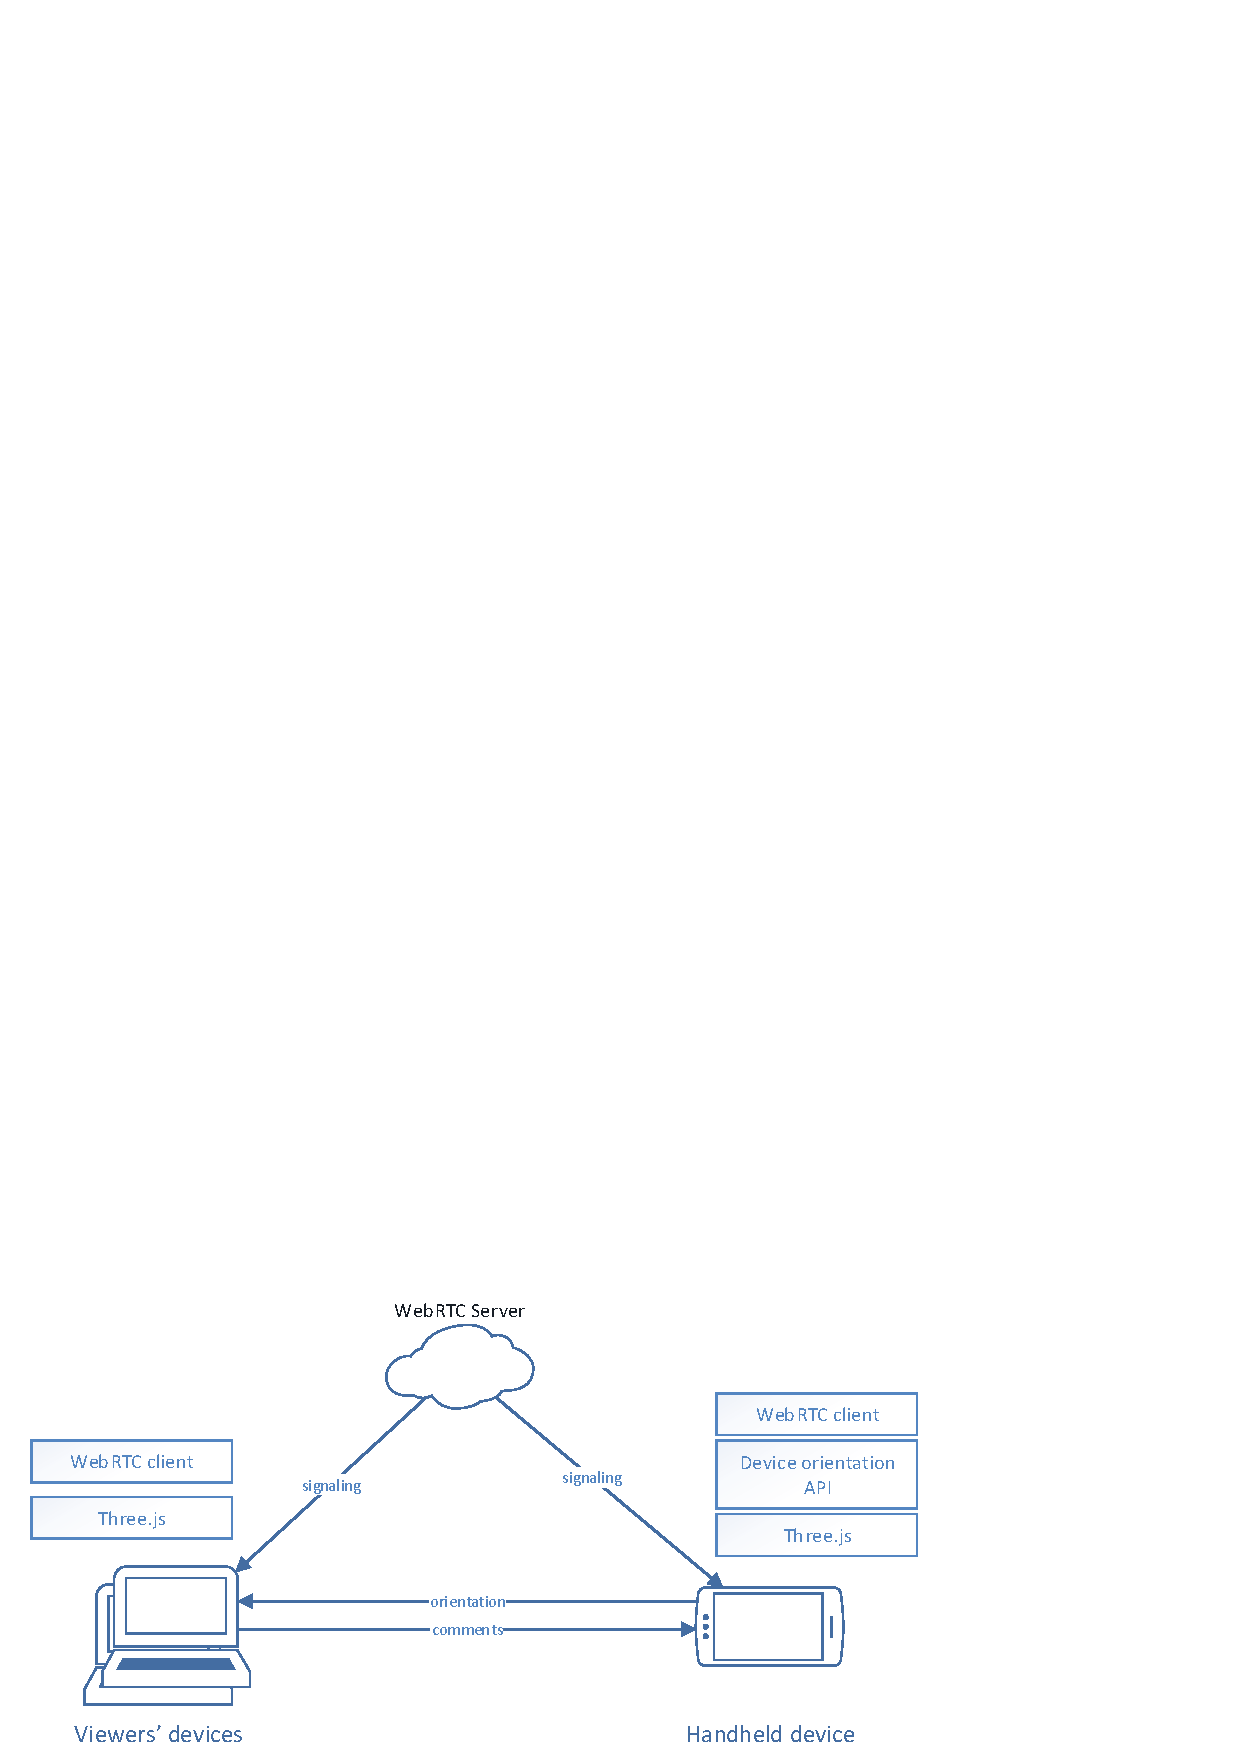
\includegraphics[width=\linewidth]{images/frontier18/system.jpg}
\caption{System components representing the sharer server-side (left) sharing with the viewer client-side (right) via WiFi: 1) the avatar position and orientation, 2) the social relationship data and 3) room and hidden components data. The system is built on Unity and runs on HoloLens.}\label{fig:frontier18:system}
\end{center}
\end{figure}

\subsection{User Study}

Using the prototype system we wanted to explore sharing different views depending on the social relationship between users, and also different methods for maintaining privacy. To do this, we conducted a pilot user study, with 12 participants (4 female) aged (25 – 43, median=32, SD=4.96). 
We asked participants to do two tasks: 

Task 1: View/share a room with or without a social proximity filter (see Figure \ref{fig:frontier18:social-filter}). In this task we had two conditions: 

\begin{itemize}
\item T1C1: Shared room without a social proximity filter where the level of details of the shared room is not affected by the social relationship between the users.
\item T1C2: Shared room with a social proximity filter where the level of details of the shared room is changed based on the social relationship between the users. 
\end{itemize}

Task 2:  The mechanism of hiding room parts for social proximity filter (see Figure \ref{fig:frontier18:hiding-mechanism}). In this task we had three conditions:

\begin{itemize}
\item T2C1: Remove – where objects are hidden by being removed from the viewer’s scene.
\item T2C2: Overlay – where objects are hidden by being overlaid by a white box. 
\item T2C3: Blur – where objects are hidden by appearing blurred to the viewer. 
\end{itemize}

Each participant tried the conditions from both sides of a viewer and a sharer. We asked participants to rate their experience after each condition. At the end of each task, we asked them to compare the conditions to each other and rank them. 

\begin{figure}
\begin{center}
\includegraphics[width=\linewidth]{images/frontier18/images-01.png}
\caption{Hiding mechanism applied on the TV screen. a) Remove, b) Overlay, c) Blur.}\label{fig:frontier18:hiding-mechanism}
\end{center}
\end{figure}


% \subsection{Experiment}

Figure \ref{fig:frontier18:setup} shows that the experiment was set up in two similar rooms so that the sharer was sharing his/her room with a remote viewer. The relative position and rotation of each user were synchronised and represented as a virtual avatar in the remote person view. The sharer could change the social relationship with the viewer by using 3-buttons (intimate, friend, stranger) situated in the middle of the room. The viewer could request the relationship to change by clicking on one of the relationship buttons. Once this happens, the sharer saw the relationship request in a different colour, which then they could approve and change the social relationship

After completing each task, we asked participants (see Table \ref{tab:frontier18:questions}) to answer three sets of Likert questionnaires; six bi-polar questions (BP), six co-presence questions (CoP) and three subjective questions (S) to measure the sense of privacy.  

\begin{table}
    \centering
    \begin{tabular}{ll}
BP1 &    Impersonal-Personal\\
BP2 &    Cold-Warm\\
BP3 &    Colourless-Colourful\\
BP4 &    Unsociable-Sociable\\
BP5 &    Closed-Open\\
BP6 &    Passive-Active\\
CoP1    &   I noticed my partner\\
CoP2    &   My partner noticed me\\
CoP3    &   My partner's presence was obvious to me\\
CoP4    &   My presence was obvious to my partner\\
CoP5    &   My partner caught my attention \\
CoP6    &   I caught my partner's attention\\
S1  & Uncomfortable-Comfortable\\
S2  & Insecure-Secure\\
S3  & Not-Interested-Interested\\
    \end{tabular}
    \caption{Subjective questions we asked participants to rate their experience on a 7-point likert scale}
    \label{tab:frontier18:questions}
\end{table}

We asked the participants open-ended questions about the strength and weakness of each condition. We also asked them to rank from most preferred to least preferred condition for each task, then explain the reason for why the chose the best and the worst condition. 

\begin{figure}
\begin{center}
\includegraphics[width=\linewidth]{images/frontier18/experiment-setup.jpg}
\caption{Experiment setup. The sharer (right) is sharing his/her 3D room with the viewer (left). The viewer sees the virtual room of the sharer overlaid on top of her/his physical room. Each user is seeing the remote person as a virtual avatar in their environment that has the position and orientation mapped to remote person.}\label{fig:frontier18:setup}
\end{center}
\end{figure}

\subsection{Results}

Figure \ref{fig:frontier18:result-filter-viewer} shows the Likert scale results for the viewer, while Figure \ref{fig:frontier18:result-filter-sharer} shows the results for the sharer. A Wilcoxon signed-rank test on the results of Task1 comparing no social filter (T1C1) and social filter (T1C2) showed that as a viewer having a social filter (T1C2) did elicit a statistically significant difference in BP5-Open (Z = -2.323, p = 0.02) and CoP1-I noticed my partner (Z =-2.066, p = 0.039). While as a sharer, having a social filter (T1C2) did elicit a statistically significant difference in CoP3-My partner's presence was obvious to me (Z = -1.993, p = 0.046) and CoP5-My partner caught my attention (Z = -2.164, p = 0.030) and S1-Comfortable (Z = -2.503, p = 0.012) and S2-Secure (Z = -2.816, p = 0.004). There was no difference in reponse to the other questions.

A Wilcoxon signed-rank test on the results of Task1 comparing no social filter (T1C1) and social filter (T1C2) showed that as a viewer having a social filter (T1C2) did elicit a statistically significant difference in BP5-Open (Z = -2.323, p = 0.02) and CoP1-I noticed my partner (Z =-2.066, p = 0.039). While as a sharer, having a social filter (T1C2) did elicit a statistically significant difference in CoP3-My partner's presence was obvious to me (Z = -1.993, p = 0.046) and CoP5-My partner caught my attention (Z = -2.164, p = 0.030) and S1-Comfortable (Z = -2.503, p = 0.012) and S2-Secure (Z = -2.816, p = 0.004).

In response to the ranking questions (Figure \ref{fig:frontier18:result-ranking}), all 12 participants preferred having a social filter when sharing room over having no filter (i.e., showing everything in the room to all social relationships). As for ranking the hiding mechanism, the most preferred option for hiding sensitive data in the room was the Remove option followed by the Overlay option, while the least preferred option was Blurring. 
We also asked participants if there was a different mechanism of hiding objects in their shared room that they would prefer (such as replacing the hidden object with a similar but less sensitive one). About 42\% thought that replacing the object was a good idea; however, most of them raised concerns about how they may not like the additional effort needed for selecting a similar object to replace.

\subsection{Discussion and Future Work}

The ranking results show that having the social filter is preferred over no social filter. However, in Likert questions, we found statistical differences in 2-5 questions out of 15. Participants with the sharer point of view had a more statistical difference than those with the viewer point of view which indicates that having a social filter is essential for people to feel comfortable regarding privacy when they have to choose. However, not as much when they have to go through the efforts of selecting which objects to hide for each social relationship.  

In the future, we would like to allow users to customise their room so that they feel more attached to the space they are sharing. In this user study, the sharer was hiding objects in the room while the viewer was observing the shared room synchronously. In the future, we can study if hiding before the viewer is connected asynchronously would affect the sense of co-presence or the feeling of being comfortable with sharing. We also would also allow participants to choose their avatars from a predefined list rather than being assigned an avatar randomly.   

\subsection{Summary}

In this paper, we described a HoloLens prototype built to share a 3D surrounding environment with social contacts, and simulate a future wearable AR social networking application; which was designed to explore how users would be willing to share views of their surroundings with remote people with different social relationships. 

We allowed users to choose which part of the room to hide or show to different social groups (intimate, friends, strangers). We run a pilot user study to test the effect of using a social filter on co-presence and the feeling of privacy from both sides as a sharer and a viewer. We found that all participants preferred having a social filter, and there was some statistical difference regarding feelings of co-presence and privacy. 

\begin{figure}
\begin{center}
\includegraphics[width=.8\linewidth]{images/frontier18/images-03.eps}
\caption{Results of social filter as viewer. *= statistically significant}\label{fig:frontier18:result-filter-viewer}
\end{center}
\end{figure}

\begin{figure}
\begin{center}
\includegraphics[width=.8\linewidth]{images/frontier18/images-04.eps}
\caption{Results of social filter as sharer. *= statistically significant}\label{fig:frontier18:result-filter-sharer}
\end{center}
\end{figure}



\begin{figure}
\begin{center}
\includegraphics[width=.9\linewidth]{images/frontier18/images-05.eps}
\caption{Results of hiding mechanism as viewer.}\label{fig:frontier18:result-hiding-viewer}
\end{center}
\end{figure}

\begin{figure}
\begin{center}
\includegraphics[width=.9\linewidth]{images/frontier18/images-06.eps}
\caption{Results of hiding mechanism as sharer.}\label{fig:frontier18:result-hiding-sharer}
\end{center}
\end{figure}

\begin{figure}
\begin{center}
\includegraphics[width=.8\linewidth]{images/frontier18/images-07.eps}
\caption{Results of ranking conditions.}\label{fig:frontier18:result-ranking}
\end{center}
\end{figure}
